\documentclass[11pt,a4paper]{article}

% --- PAQUETES FUNDAMENTALES Y TIPOGRAFÍA ---
\usepackage[utf8]{inputenc}
\usepackage[spanish,es-tabla]{babel}
\usepackage{amsmath,amsfonts,amssymb,bm}
\usepackage{geometry}
\geometry{top=2.5cm, bottom=2.5cm, left=2.5cm, right=2.5cm}
\usepackage{booktabs}
\usepackage{multirow}
\usepackage{graphicx}
\usepackage{listings}
\usepackage{xcolor}
\usepackage{hyperref}
\usepackage{microtype}
\usepackage{cite}
\usepackage{authblk}

% --- CONFIGURACIÓN DE HIPERVÍNCULOS ---
\hypersetup{
    colorlinks=true,
    linkcolor=blue!80!black,
    citecolor=blue!80!black,
    urlcolor=blue!70!black
}

% --- CONFIGURACIÓN DE LISTINGS PARA CÓDIGO PYTHON ---
\definecolor{codegreen}{rgb}{0,0.6,0}
\definecolor{codegray}{rgb}{0.5,0.5,0.5}
\definecolor{codepurple}{rgb}{0.58,0,0.82}
\definecolor{backcolour}{rgb}{0.97,0.97,0.97}

\lstdefinestyle{pythonstyle}{
    backgroundcolor=\color{backcolour},   
    commentstyle=\color{codegreen}\itshape,
    keywordstyle=\color{blue}\bfseries,
    numberstyle=\tiny\color{codegray},
    stringstyle=\color{codepurple},
    basicstyle=\ttfamily\footnotesize,
    breakatwhitespace=false,         
    breaklines=true,                 
    captionpos=b,                    
    keepspaces=true,                 
    numbers=left,                    
    numbersep=5pt,                  
    showspaces=false,                
    showstringspaces=false,
    showtabs=false,                  
    tabsize=4,
    frame=single,
    rulecolor=\color{gray!30}
}
\lstset{style=pythonstyle}

% --- METADATOS DEL DOCUMENTO ---
\title{\textbf{\Large Evaluación Experimental del Algoritmo de Viterbi frente a Clasificadores Estáticos en la Inferencia de Regímenes Sísmicos Latentes: Un Estudio Metodológico de Simulación Computacional}}

% AUTOR: Únicamente Francisco Javier Florez Ramirez (estudiante).
% El Dr. Loaiza López figura como Docente Asesor/Tutor, NO como coautor del artículo.
\author{\textbf{Francisco Javier Florez Ramirez}}

\affil{Estudiante de Ingeniería de Software y Datos, Curso de Simulación,\\
Institución Universitaria Digital de Antioquia (IU Digital), Medellín, Colombia.\\
Correo: \texttt{francisco.florez@est.iudigital.edu.co}\\[4pt]
\textit{Docente Asesor:} Dr. Julián Andrés Loaiza López,
Departamento de Ingeniería de Software y Datos, IU Digital.\\
Correo: \texttt{julian.loaiza@prof.iudigital.edu.co}}

\date{\today}

\begin{document}

\maketitle

\begin{abstract}
\noindent La inferencia de regímenes dinámicos latentes en fenómenos geofísicos a partir de observaciones de superficie constituye un reto fundamental en ciencias de la ingeniería. Cuando las magnitudes sísmicas continuas se transforman en categorías ordinales discretas (Baja, Media y Alta), surgen regiones de ambigüedad estocástica donde estados distintos presentan probabilidades de emisión idénticas. Este trabajo evalúa de manera comparativa la capacidad del algoritmo de Viterbi en un Modelo Oculto de Markov (HMM) discreto frente a dos clasificadores estáticos que prescinden de la modelación temporal: un clasificador reactivo por máxima emisión directa y un clasificador bayesiano puntual estático con distribución a priori fija. El diseño experimental adopta un enfoque híbrido sobre parámetros hipotéticos conocidos $\lambda = (A, B, \pi)$: una fase analítica sobre una secuencia representativa de cinco eventos ($T = 5$) y una fase inferencial basada en $N = 100$ realizaciones independientes generadas por simulación Monte Carlo ($T = 50$, \texttt{seed = 42}). Los resultados verificados demuestran que el clasificador reactivo presenta un empate exacto que exige una convención de desempate ($P = 0.50$) ante magnitudes medias y que el clasificador bayesiano estático colapsa en una predicción constante de reposo por sesgo del prior ($\pi_1 = 0.80$). En contraste, el algoritmo de Viterbi reconstruye retrospectivamente la trayectoria hacia el camino gradual $(\text{Reposo}, \text{Reposo}, \text{Actividad Menor}, \text{Enjambre}, \text{Enjambre})$, alcanzando la mayor log-verosimilitud conjunta ($-7.2538$ frente a $-7.4361$ y $-8.9453$). En la evaluación estadística, Viterbi obtuvo una precisión media del $72.62\%$ con un intervalo de confianza al 95\,\% de $[70.48\%, 74.76\%]$, obteniendo una precisión media mayor que la del modelo bayesiano estático ($61.54\%$) y aventajando al clasificador por máxima emisión ($69.72\%$). Se concluye que la modelación de transiciones temporales es determinante para regularizar la inferencia ante observaciones solapadas en sistemas estocásticos simulados.
\vspace{0.3cm}

\noindent \textbf{Palabras clave:} Modelos Ocultos de Markov (HMM), Algoritmo de Viterbi, Simulación Estocástica, Ambigüedad Observacional, Inferencia Secuencial, Intervalos de Confianza al 95\,\%.
\end{abstract}

\hrule
\vspace{0.4cm}

\section{Introducción}

El modelado y evaluación de sistemas estocásticos complejos en ciencias de la ingeniería frecuentemente enfrenta el desafío de inferir la dinámica interna de procesos cuyos estados verdaderos no son directamente accesibles mediante instrumentación superficial. En tales escenarios, las observaciones adquiridas operan como señales indirectas, discretizadas o corrompidas por ruido observacional. Dentro de este paradigma, los Modelos Ocultos de Markov (\textit{Hidden Markov Models}, HMM) constituyen un marco formal probabilístico y computacional robusto para desacoplar los estados latentes de sus emisiones manifiestas~\cite{baum1970maximization, rabiner1989tutorial}.

Desde la perspectiva de la metodología de simulación computacional, la formulación de estos modelos requiere trascender la mera adopción teórica para cumplir con estándares rigurosos de reproducibilidad, cuantificación de la incertidumbre y análisis comparativo de sensibilidad. En contextos de monitoreo de fenómenos geodinámicos y eventos físicos secuenciales, la discretización de variables continuas en categorías ordinales (como magnitudes bajas, medias o altas) introduce regiones de incertidumbre epistémica en las que distintos estados del sistema poseen capacidades de emisión solapadas. El presente trabajo investiga cómo la modelación explícita de la memoria temporal permite resolver dichas indeterminaciones frente a métodos convencionales de clasificación puntual e independiente.

\subsection{Planteamiento del Problema y Delimitación}

Muchos sistemas en ingeniería presentan transiciones de estado latentes gobernadas por una inercia física determinada, pero cuya supervisión descansa en sensores que registran lecturas aisladas a lo largo del tiempo. En una estación de monitoreo que registra eventos en orden cronológico, el estado de reactivación o reposo de la fuente generadora debe deducirse a partir del nivel de magnitud del evento observado. Sin embargo, cuando se emplean clasificadores heurísticos, reactivos o puramente estáticos, la inferencia sufre dos fallas metodológicas fundamentales:

\begin{enumerate}
    \item \textbf{Ambigüedad por solapamiento de emisiones:} Si dos regímenes físicos distintos (por ejemplo, una fase de actividad menor y una fase precursora de enjambre) comparten una probabilidad equivalente de emitir una observación intermedia (magnitud media), el clasificador por máxima emisión presenta un empate y requiere una convención. En este experimento selecciona el primer índice, s2. El clasificador bayesiano estático pondera las emisiones por el prior y obtiene un máximo único en s1 ante magnitud media.
    \item \textbf{Rigidez e inercia del sesgo a priori:} Si el clasificador integra una distribución a priori fija sin un mecanismo recursivo de actualización dinámica de transiciones, la alta prevalencia de un estado de reposo inicial enmascara y neutraliza la evidencia de eventos moderados o extremos sucesivos, conduciendo a diagnósticos sistemáticamente sesgados.
\end{enumerate}

\noindent \textbf{Delimitación del alcance:} En estricto apego a las directrices de integridad científica, este estudio se delimita a una investigación metodológica basada en simulación estocástica controlada con parámetros hipotéticos conocidos $\lambda = (A, B, \pi)$. El estudio no constituye una caracterización sismológica de campo ni pretende validar la física de una falla tectónica específica mediante catálogos instrumentales reales, ya que las etiquetas de estado analizadas (Reposo Sísmico, Actividad Menor y Enjambre Sísmico) representan categorías hipotéticas de simulación.

El diseño experimental adopta un enfoque híbrido:
\begin{enumerate}
    \item[a)] Una evaluación determinista paso a paso sobre una secuencia ordinal representativa de cinco eventos (Baja, Baja, Media, Media, Alta), aislando analíticamente la celosía de programación dinámica y desambiguación del Algoritmo de Viterbi.
    \item[b)] Una evaluación estadística estandarizada basada en $N = 100$ réplicas sintéticas independientes generadas por simulación Monte Carlo con longitud de secuencia fija de $T = 50$ pasos bajo semilla constante (\texttt{seed = 42}), reportando promedios, desviaciones estándar e intervalos de confianza del 95\,\% ($IC_{95\%}$) para contrastar cuantitativamente la precisión de decodificación y estabilidad frente a los baselines de control.
\end{enumerate}

\subsection{Preguntas de Investigación}

Para orientar la investigación y estructurar el aporte del trabajo sin presuponer superioridad del modelo propuesto, se definen dos preguntas investigables con comparación explícita y criterios objetivos de evaluación:

\begin{itemize}
    \item \textbf{P1 (Comparación Analítica y Desambiguación en Secuencia Base):} ¿Cómo difieren la trayectoria de estados latentes inferida y la log-verosimilitud conjunta $\log P(\mathcal{O}, \hat{S} \mid \lambda)$ obtenidas mediante el algoritmo de Viterbi frente a clasificadores puntuales (máxima emisión directa y bayesiano estático) al procesar una secuencia sísmica discreta que presenta emisiones idénticas para regímenes dinámicos distintos?
    \item \textbf{P2 (Comparación Estadística y Estabilidad bajo Simulación Monte Carlo):} ¿Qué diferencias cuantitativas existen en la precisión media de decodificación y en sus intervalos de confianza al 95\,\% ($IC_{95\%}$) entre el algoritmo de Viterbi y clasificadores estáticos sin memoria, al ser evaluados sobre $N = 100$ realizaciones estocásticas sintéticas independientes de longitud $T = 50$ generadas por el mismo modelo $\lambda$?
\end{itemize}

\subsection{Objetivos y Aportes del Trabajo}

\textbf{Objetivo General:} Evaluar de manera comparativa la consistencia y precisión en la inferencia de estados geodinámicos latentes del algoritmo de Viterbi frente a clasificadores estáticos puntuales, mediante el análisis analítico de secuencias con emisiones ambiguas y la simulación Monte Carlo de series estocásticas sintéticas con parámetros conocidos.

\textbf{Objetivos Específicos:}
\begin{enumerate}
    \item Determinar la trayectoria de estados latentes y calcular la log-verosimilitud conjunta del camino inferido por el algoritmo de Viterbi, el clasificador por máxima emisión directa y el clasificador bayesiano estático sobre una secuencia discreta de cinco eventos, analizando el comportamiento de cada método ante observaciones con emisiones intermedias solapadas.
    \item Cuantificar la precisión de decodificación, su dispersión y sus intervalos de confianza al 95\,\% ($IC_{95\%}$) para los tres modelos en un entorno de simulación Monte Carlo con 100 secuencias sintéticas independientes de 50 pasos de tiempo, describiendo las diferencias de precisión y su incertidumbre entre métodos.
\end{enumerate}

\textbf{Aportes Principales:}
\begin{enumerate}
    \item Formalismo matemático unificado y trazable adaptado a la inferencia de regímenes sísmicos latentes bajo el estándar institucional de simulación.
    \item Evaluación comparativa reproducible de un decodificador secuencial y dos clasificadores puntuales sobre las mismas observaciones.
    \item Suite de código determinista en Python (\texttt{seed = 42}) que garantiza la reproducibilidad total de los experimentos analíticos y de Monte Carlo.
\end{enumerate}

\section{Estado del Arte}

La fundamentación teórica de los Modelos Ocultos de Markov se originó en la formulación estocástica de Baum et al.~\cite{baum1970maximization} y fue estructurada algorítmicamente para ingeniería por Rabiner~\cite{rabiner1989tutorial}. En la literatura sismológica y geofísica reciente, los HMM han adquirido protagonismo para modelar procesos subterráneos no observables (como la acumulación de esfuerzo y la reactivación de fallas) a partir de secuencias de eventos en superficie. 

Como referencia contemporánea de articulación, el estudio de Georgakopoulou et al.~\cite{georgakopoulou2024seismic} aborda la evaluación de sismicidad en América Central y del Sur implementando modelos de Poisson ocultos (PHMM) para caracterizar transiciones entre estados latentes de quietud y crisis sísmicas en catálogos extensos. De manera complementaria, investigaciones recientes han empleado HMMs para modelar la recurrencia de sismos de baja frecuencia (Allen y Wang~\cite{allen2023hidden}), la inferencia de niveles de sismicidad mediante cambios de régimen de Markov (Zhang et al.~\cite{zhang2023statistical}), y la ocurrencia de eventos sísmicos en entornos urbanos y arcos tectónicos (Felix et al.~\cite{felix2022poisson}, Endrayanto et al.~\cite{endrayanto2026markov}, Bountzis et al.~\cite{bountzis2022pseudo}). Asimismo, se ha explorado la generación de catálogos sintéticos con cadenas de Markov (Karaca~\cite{karaca2021generation}), el análisis segmental de megacabalgamientos (Rizal et al.~\cite{rizal2023seismic}), la aplicación de Viterbi para decodificar estados de esfuerzo en el Mar Egeo (Danisman y Kocer~\cite{danisman2021fitting}) y el modelado de patrones espacio-temporales de sismicidad en zonas de subducción (Benali et al.~\cite{benali2020modelling}).

A pesar de esta proliferación de aplicaciones, los trabajos existentes se concentran en catálogos empíricos con observaciones ricas o continuas. Persiste un vacío metodológico en la evaluación analítica del comportamiento del algoritmo de Viterbi cuando las magnitudes se discretizan en un número pequeño de categorías ordinales que presentan probabilidades de emisión exactamente idénticas entre estados distintos. En la Tabla~\ref{tab:estado_arte} se resume la comparación frente a las aproximaciones clave.

\begin{table}[htbp]
\centering
\small
\caption{Tabla comparativa de trabajos previos en modelado markoviano y localización del vacío de investigación.}
\label{tab:estado_arte}
\begin{tabular}{p{3.2cm}p{3.2cm}p{2.6cm}p{2.6cm}p{3.4cm}}
\toprule
\textbf{Referencia} & \textbf{Dominio / Enfoque} & \textbf{Variante HMM} & \textbf{Métricas} & \textbf{Vacío frente a este Trabajo} \\
\midrule
Baum et al. (1970)~\cite{baum1970maximization} & Fundamentación teórica & DTMC oculta general & Maximización EM & Sin baselines de control ni simulación determinista. \\
Rabiner (1989)~\cite{rabiner1989tutorial} & Procesamiento de voz & HMM discreto 1.er orden & Viterbi / Forward & Enfoque canónico; no examina empates exactos en baja cardinalidad. \\
Georgakopoulou et al. (2024)~\cite{georgakopoulou2024seismic} & Sismicidad Centro y Suramérica & Poisson-HMM regional & Estimación paramétrica & Ajuste en catálogos masivos; no aísla el aporte marginal de Viterbi. \\
Allen \& Wang (2023)~\cite{allen2023hidden} & Sismos de baja frecuencia & HMM eventos raros & Tasa de transición & Modela recurrencia continua sin contrastar sesgos a priori. \\
Danisman \& Kocer (2021)~\cite{danisman2021fitting} & Sismos en el Mar Egeo & HMM con decodificación & Reconstrucción de estados & No evalúa desambiguación ante emisiones intermedias idénticas. \\
\textbf{Este Trabajo (2026)} & \textbf{Simulación en ingeniería} & \textbf{HMM Discreto (Viterbi)} & \textbf{Log-verosimilitud, Precisión ($IC_{95\%}$)} & \textbf{Compara decodificación secuencial y clasificación puntual ante emisiones ambiguas.} \\
\bottomrule
\end{tabular}
\end{table}

\subsection{Identificación del Vacío de Investigación}

A partir de la revisión sistemática se constata que:
\begin{enumerate}
    \item Las investigaciones contemporáneas~\cite{georgakopoulou2024seismic, allen2023hidden, zhang2023statistical, danisman2021fitting} demuestran la validez conceptual de asociar estados latentes de Markov a regímenes geodinámicos (como reposo, aceleración o enjambres).
    \item Sin embargo, no se ha evaluado cómo se comporta la decodificación secuencial en presencia de solapamiento estocástico total ($B_{2,2} = B_{3,2} = 0.50$) frente a clasificadores reactivos (que sufren indeterminación) y bayesianos estáticos (que colapsan por dominancia de $\pi_1 = 0.80$).
\end{enumerate}

Este trabajo llena dicho vacío mediante un diseño experimental de doble capa: trazabilidad paso a paso sobre una secuencia base representativa ($T=5$) y evaluación estadística mediante $N=100$ réplicas Monte Carlo ($T=50$, \texttt{seed=42}) con intervalos de confianza al 95\,\% ($IC_{95\%}$).

\section{Marco Teórico}

\subsection{Distribuciones de Probabilidad en Modelos Secuenciales Discretos}

Los modelos secuenciales estocásticos caracterizan la probabilidad de transiciones y emisiones sobre variables aleatorias continuas o discretas. En el contexto de este trabajo, la señal observable continua (magnitud sismológica) se discretiza en una variable ordinal perteneciente a un alfabeto finito $V = \{v_1, v_2, v_3\}$. Cada estado latente $s_j$ rige la generación de observaciones mediante una distribución categórica o multinomial sobre dicho alfabeto, definida por la función de masa de probabilidad:
\begin{equation}
b_j(k) = P(O_t = v_k \mid S_t = s_j), \quad \text{con } \sum_{k=1}^M b_j(k) = 1, \quad \forall j \in \{1, \dots, N\}
\end{equation}

La formalización de los umbrales cuantitativos de discretización se define rigurosamente como:
\begin{itemize}
    \item $v_1$ (\textbf{Magnitud Baja}): Magnitud sísmica $M < 3.0$.
    \item $v_2$ (\textbf{Magnitud Media}): Magnitud sísmica $3.0 \le M \le 5.0$ (ambos límites incluidos).
    \item $v_3$ (\textbf{Magnitud Alta}): Magnitud sísmica $M > 5.0$.
\end{itemize}

\subsection{Cadenas de Markov y Propiedad de Markov}

Una Cadena de Markov de Tiempo Discreto (DTMC) es una secuencia de variables aleatorias $\{S_t\}_{t=1}^T$ en un espacio de estados finito $S = \{s_1, \dots, s_N\}$ que satisface la propiedad de memoria corta de primer orden:
\begin{equation}
P(S_t = s_j \mid S_{t-1} = s_i, S_{t-2} = s_{i_{t-2}}, \dots, S_1 = s_{i_1}) = P(S_t = s_j \mid S_{t-1} = s_i) = A_{i,j}
\end{equation}

Esta propiedad postula que el estado futuro del sistema depende exclusivamente del estado presente inmediato, siendo condicionalmente independiente de la historia pasada de transiciones.

\subsection{Formalización del Modelo Oculto de Markov (HMM)}

\begin{figure}[htbp]
\centering
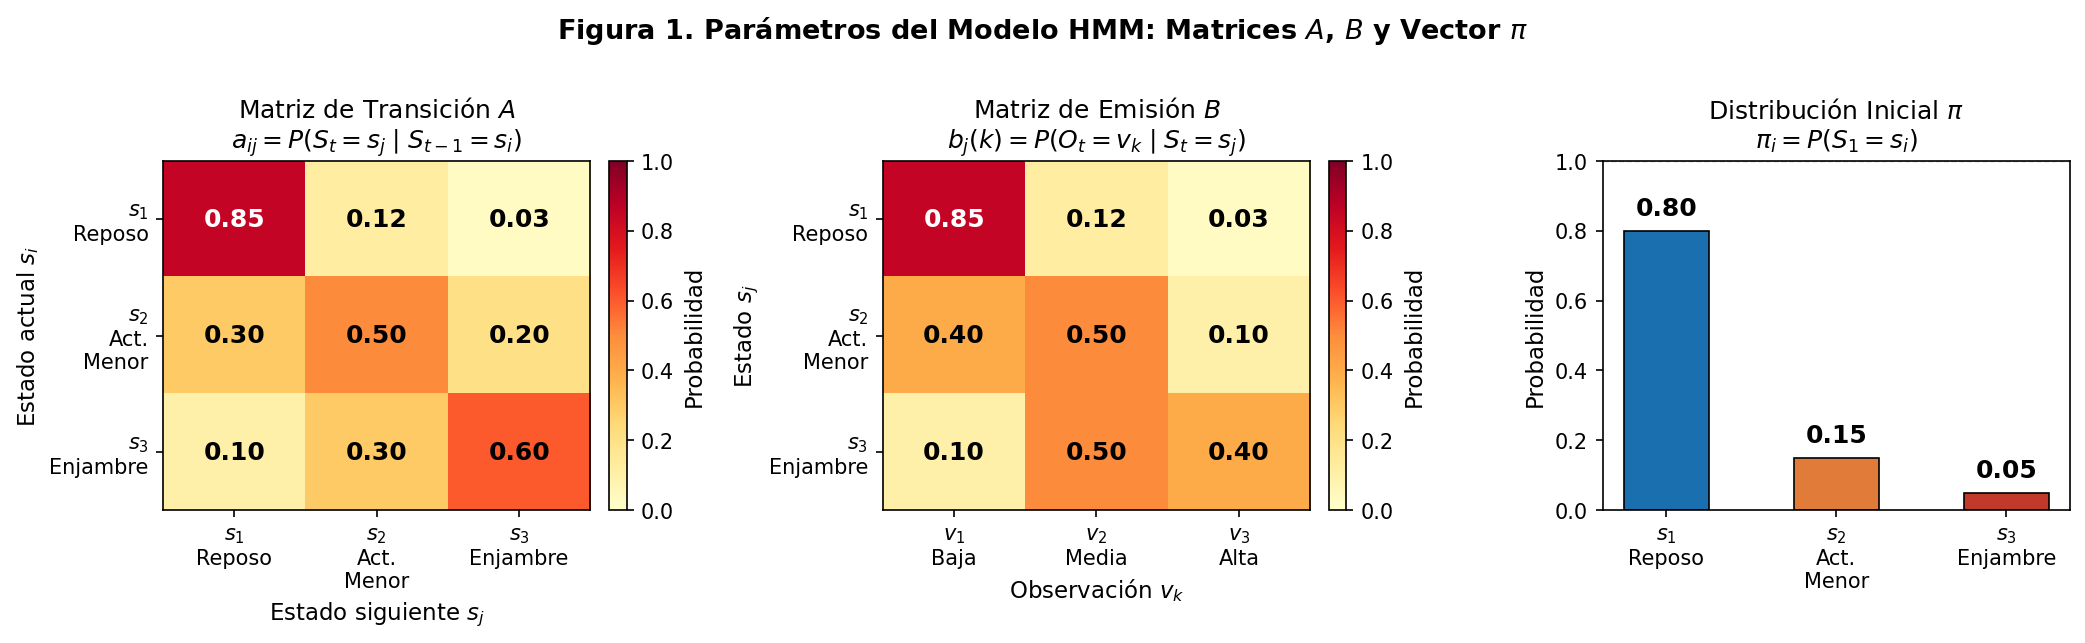
\includegraphics[width=\textwidth]{figures/fig1_matrices_hmm.png}
\caption{Representación visual de los parámetros canónicos del modelo $\lambda = (A, B, \pi)$. Izquierda: matriz de transición $A$ — el Reposo Sísmico ($s_1$) presenta alta auto-persistencia (0.85). Centro: matriz de emisión $B$ — los estados $s_2$ y $s_3$ comparten probabilidad idéntica (0.50) ante magnitudes medias ($v_2$), lo cual genera la ambigüedad estocástica central del estudio. Derecha: vector inicial $\pi$ — el sesgo dominante hacia $s_1$ (0.80) es la causa del colapso del clasificador bayesiano estático.}
\label{fig:matrices}
\end{figure}

Un Modelo Oculto de Markov discreto de primer orden se define formalmente mediante la tupla quintupla:
\begin{equation}
\lambda = (S, V, A, B, \pi)
\end{equation}
donde:
\begin{itemize}
    \item $S = \{s_1, s_2, s_3\}$ es el conjunto finito de $N = 3$ estados latentes o no observables:
    \begin{itemize}
        \item $s_1$: Reposo Sísmico (fase tectónica de quietud o acumulación de esfuerzo basal).
        \item $s_2$: Actividad Menor (fracturación localizada de microfallas con liberación energética moderada).
        \item $s_3$: Enjambre Sísmico (aceleración co-sísmica o crisis de sismicidad concentrada).
    \end{itemize}
    \item $V = \{v_1, v_2, v_3\}$ es el conjunto finito de $M = 3$ símbolos observables discretizados (Magnitud Baja, Media y Alta).
    \item $A \in \mathbb{R}^{N \times N}$ es la matriz de probabilidades de transición temporal entre estados latentes, cuyos elementos satisfacen la condición estocástica por filas:
    \begin{equation}
    A_{i,j} = P(S_t = s_j \mid S_{t-1} = s_i), \quad A_{i,j} \ge 0, \quad \sum_{j=1}^N A_{i,j} = 1, \quad \forall i \in \{1, \dots, N\}
    \end{equation}
    Parametrización del caso experimental:
    \begin{equation}
    A = \begin{pmatrix}
    0.85 & 0.12 & 0.03 \\
    0.30 & 0.50 & 0.20 \\
    0.10 & 0.30 & 0.60
    \end{pmatrix}
    \end{equation}
    \textit{Verificación de cierre estocástico:}
    Fila 1: $0.85 + 0.12 + 0.03 = 1.000$; 
    Fila 2: $0.30 + 0.50 + 0.20 = 1.000$; 
    Fila 3: $0.10 + 0.30 + 0.60 = 1.000$.
    \item $B \in \mathbb{R}^{N \times M}$ es la matriz de probabilidades de emisión, donde cada componente cuantifica la probabilidad condicional de observar el símbolo $v_k$ dado que el sistema se halla en el estado $s_j$:
    \begin{equation}
    B_{j,k} = P(O_t = v_k \mid S_t = s_j), \quad B_{j,k} \ge 0, \quad \sum_{k=1}^M B_{j,k} = 1, \quad \forall j \in \{1, \dots, N\}
    \end{equation}
    Parametrización del caso experimental:
    \begin{equation}
    B = \begin{pmatrix}
    0.85 & 0.12 & 0.03 \\
    0.40 & 0.50 & 0.10 \\
    0.10 & 0.50 & 0.40
    \end{pmatrix}
    \end{equation}
    \textit{Verificación de cierre estocástico:}
    Fila 1: $0.85 + 0.12 + 0.03 = 1.000$; 
    Fila 2: $0.40 + 0.50 + 0.10 = 1.000$; 
    Fila 3: $0.10 + 0.50 + 0.40 = 1.000$.
    \item $\pi \in \mathbb{R}^N$ es la distribución de probabilidad inicial del sistema en el instante $t = 1$:
    \begin{equation}
    \pi_i = P(S_1 = s_i), \quad \pi_i \ge 0, \quad \sum_{i=1}^N \pi_i = 1
    \end{equation}
    Parametrización del caso experimental:
    \begin{equation}
    \pi = (0.80, \quad 0.15, \quad 0.05)
    \end{equation}
    \textit{Verificación:} $0.80 + 0.15 + 0.05 = 1.000$.
\end{itemize}

\subsection{Los Tres Problemas Clásicos en HMM y Distinción Funcional}

Siguiendo la taxonomía clásica de Rabiner~\cite{rabiner1989tutorial}, la teoría de HMM se articula en torno a tres problemas fundamentales:
\begin{enumerate}
    \item \textbf{Problema 1: Evaluación o Verosimilitud (Forward / Backward):} Dada la secuencia de observaciones $\mathcal{O} = (O_1, \dots, O_T)$ y el modelo $\lambda$, calcular la probabilidad marginal $P(\mathcal{O} \mid \lambda) = \sum_{\text{todas las } S} P(\mathcal{O}, S \mid \lambda)$.
    \item \textbf{Problema 2: Decodificación de Estados Latentes (Algoritmo de Viterbi):} Dada la secuencia observada $\mathcal{O}$ y el modelo $\lambda$, hallar la secuencia óptima completa de estados ocultos $\hat{S} = (\hat{s}_1, \dots, \hat{s}_T)$ que maximice la probabilidad conjunta:
    \begin{equation}
    \hat{S} = \arg\max_{S} P(\mathcal{O}, S \mid \lambda)
    \end{equation}
    \item \textbf{Problema 3: Aprendizaje y Ajuste Paramétrico (Baum-Welch / EM):} A partir de observaciones no etiquetadas $\mathcal{O}$, estimar el conjunto de parámetros $\lambda^* = \arg\max_\lambda P(\mathcal{O} \mid \lambda)$.
\end{enumerate}

\noindent \textbf{Justificación metodológica del enfoque adoptado:} El presente trabajo se enfoca de manera exclusiva y rigurosa en el \textbf{Problema 2 (Decodificación)}, evaluado a través del Algoritmo de Viterbi. Debido a que el caso de estudio proporciona una parametrización de referencia hipotética completa $\lambda = (A, B, \pi)$, la estimación por Baum-Welch (Problema 3) resulta innecesaria y contraproducente sobre una secuencia corta de cinco datos, donde los estimadores de máxima verosimilitud convergerían a distribuciones degeneradas.

\section{Metodología e Implementación}

\subsection{Unidades de Análisis y Protocolo Experimental}

La metodología experimental se estructura en dos fases complementarias de evaluación:

\begin{enumerate}
    \item \textbf{Fase 1: Evaluación Analítica Determinista ($T = 5$):} Se analiza la secuencia base representativa del caso experimental:
    \begin{equation}
    \mathcal{O} = (\text{Baja}, \text{Baja}, \text{Media}, \text{Media}, \text{Alta}) \equiv (v_1, v_1, v_2, v_2, v_3)
    \end{equation}
    En esta fase se calcula manualmente y mediante software la celosía de programación dinámica de Viterbi, comparando su log-verosimilitud y secuencia inferida contra los baselines de control.
    \item \textbf{Fase 2: Evaluación Estadística Inferencial por Simulación Monte Carlo ($N = 100, T = 50$):} Para cuantificar la variación entre secuencias sintéticas, se generan 100 realizaciones sintéticas independientes del proceso markoviano bajo el modelo $\lambda = (A, B, \pi)$. Cada realización genera tanto el estado latente verdadero $S_t^*$ (\textit{ground truth} de simulación) como la emisión observable $O_t$. Se decodifica la secuencia con cada modelo y se cuantifica la precisión, desviación estándar e intervalo de confianza del 95\,\%.
\end{enumerate}

\subsection{Modelos de Contraste y Control Experimental}

Para comparar la decodificación secuencial con reglas puntuales, se implementaron dos baselines estáticos sin memoria. Los métodos difieren en objetivo, prior y acceso a la secuencia completa; la comparación no aísla el efecto de A por separado:

\begin{itemize}
    \item \textbf{Baseline 1: Clasificador Reactivo por Máxima Emisión Directa:}
    Asigna el estado latente en cada instante de tiempo evaluando únicamente la verosimilitud de emisión de la observación presente, ignorando el orden temporal y la historia previa:
    \begin{equation}
    \hat{s}_t^{(B1)} = \arg\max_{j \in \{1, \dots, N\}} P(O_t \mid S_t = s_j) = \arg\max_{j} B_{j, k(t)}
    \end{equation}
    \item \textbf{Baseline 2: Clasificador Bayesiano Puntual Estático:}
    Incorpora la distribución a priori inicial del sistema $\pi$, pero opera de forma estática en cada punto ignorando las transiciones dinámicas entre instantes adyacentes:
    \begin{equation}
    \hat{s}_t^{(B2)} = \arg\max_{j \in \{1, \dots, N\}} \pi_j \cdot P(O_t \mid S_t = s_j) = \arg\max_{j} \left( \pi_j \cdot B_{j, k(t)} \right)
    \end{equation}
\end{itemize}

\noindent \textbf{Configuración reproducible:} Se inicializa una sola instancia local de \texttt{numpy.random.RandomState(42)} (MT19937). En cada evento se sortea el estado y después su emisión; no se reinicia la semilla entre réplicas. B1 resuelve empates por el primer índice ($s_2$ ante magnitud media) en ambas fases. Se usa desviación muestral (\texttt{ddof=1}) e intervalo normal aproximado $\bar{X}\pm1.96s/\sqrt{N}$. No se calcula un valor p ni se sustituye una prueba pareada por intervalos individuales. La ejecución se verificó con Python 3.13.3 y NumPy 2.3.3.

\subsection{Prevención de Fuga de Información (\textit{Data Leakage})}

En la simulación Monte Carlo, la generación de las trayectorias sintéticas sigue el flujo causal forward: el estado $S_t$ se genera a partir de $S_{t-1}$ mediante $A$, y la observación $O_t$ se genera condicionalmente a $S_t$ mediante $B$. Los modelos decodificadores reciben únicamente la secuencia observable $\mathcal{O}$ y el parámetro $\lambda$; en ningún momento del cómputo los algoritmos tienen acceso a la secuencia latente oculta $S^*$, la cual se reserva exclusivamente para la evaluación ex-post de precisión.

\subsection{Implementación Algorítmica en Python}

El algoritmo de Viterbi opera mediante programación dinámica sobre las probabilidades de camino parcial máximo $\delta_t(j)$ y los punteros de retroceso $\psi_t(j)$:
\begin{enumerate}
    \item \textbf{Inicialización ($t = 1$):}
    \begin{equation}
    \delta_1(j) = \pi_j \cdot B_{j, k(1)}, \quad \psi_1(j) = 0, \quad \forall j \in \{1, \dots, N\}
    \end{equation}
    \item \textbf{Recursión ($t = 2, \dots, T$):}
    \begin{align}
    \delta_t(j) &= \max_{1 \le i \le N} \left[ \delta_{t-1}(i) \cdot A_{i,j} \right] \cdot B_{j, k(t)} \\
    \psi_t(j) &= \arg\max_{1 \le i \le N} \left[ \delta_{t-1}(i) \cdot A_{i,j} \right]
    \end{align}
    \item \textbf{Terminación y Retroceso (\textit{Backtracking}):}
    \begin{align}
    P^* &= \max_{1 \le j \le N} \delta_T(j), \quad \hat{s}_T = \arg\max_{1 \le j \le N} \delta_T(j) \\
    \hat{s}_t &= \psi_{t+1}(\hat{s}_{t+1}), \quad \text{para } t = T-1, T-2, \dots, 1
    \end{align}
\end{enumerate}

En el Listado~\ref{lst:viterbi} se muestra el uso de \texttt{src/hmm\_model.py} y \texttt{src/experimento.py}. El script \texttt{run\_viterbi\_caso.py} es el punto de entrada y exporta los resultados.

\begin{lstlisting}[language=Python, caption={Uso del núcleo y ejecución del experimento reproducible.}, label={lst:viterbi}]
from src.hmm_model import A, B, PI, OBS_BASE, viterbi
from src.experimento import run_experiment, export_results

path, log_prob, delta, psi = viterbi(OBS_BASE, A, B, PI)
report, records = run_experiment(N_runs=100, T=50, seed=42)
export_results(report, records, "resultados")
\end{lstlisting}

\section{Resultados y Análisis Estadístico}

\subsection{Evolución Analítica de la Celosía de Viterbi sobre la Secuencia Base ($T=5$)}

Se evaluó la secuencia Baja, Baja, Media, Media y Alta con las matrices del caso didáctico. La Tabla~\ref{tab:celosia_viterbi} presenta los valores calculados por el núcleo común.

\begin{table}[htbp]
\centering
\small
\caption{Probabilidades de camino parcial máximo y predecesores. Los índices de $\psi$ comienzan en cero.}
\label{tab:celosia_viterbi}
\begin{tabular}{clrrrl}
\toprule
$t$ & Observación & $\delta_t(s_1)$ & $\delta_t(s_2)$ & $\delta_t(s_3)$ & $\psi_t$ \\
\midrule
1 & Baja & 0.680000000 & 0.060000000 & 0.005000000 & [0, 0, 0] \\
2 & Baja & 0.491300000 & 0.032640000 & 0.002040000 & [0, 0, 0] \\
3 & Media & 0.050112600 & 0.029478000 & 0.007369500 & [0, 0, 0] \\
4 & Media & 0.005111485 & 0.007369500 & 0.002947800 & [0, 1, 1] \\
5 & Alta & 0.000130343 & 0.000368475 & 0.000707472 & [0, 1, 2] \\
\bottomrule
\end{tabular}
\end{table}

El retroceso desde $s_3$ en el quinto evento recupera $(s_1,s_1,s_2,s_3,s_3)$. El camino óptimo puede diferir de los máximos locales de $\delta_t$; la reconstrucción utiliza la secuencia completa.
\begin{equation}
P^*=0.000707472,\qquad \ln P^*=\ln(0.000707472)=-7.2538.
\end{equation}

\subsection{Contraste frente a los Baselines en la Secuencia Base}

\begin{figure}[htbp]
\centering
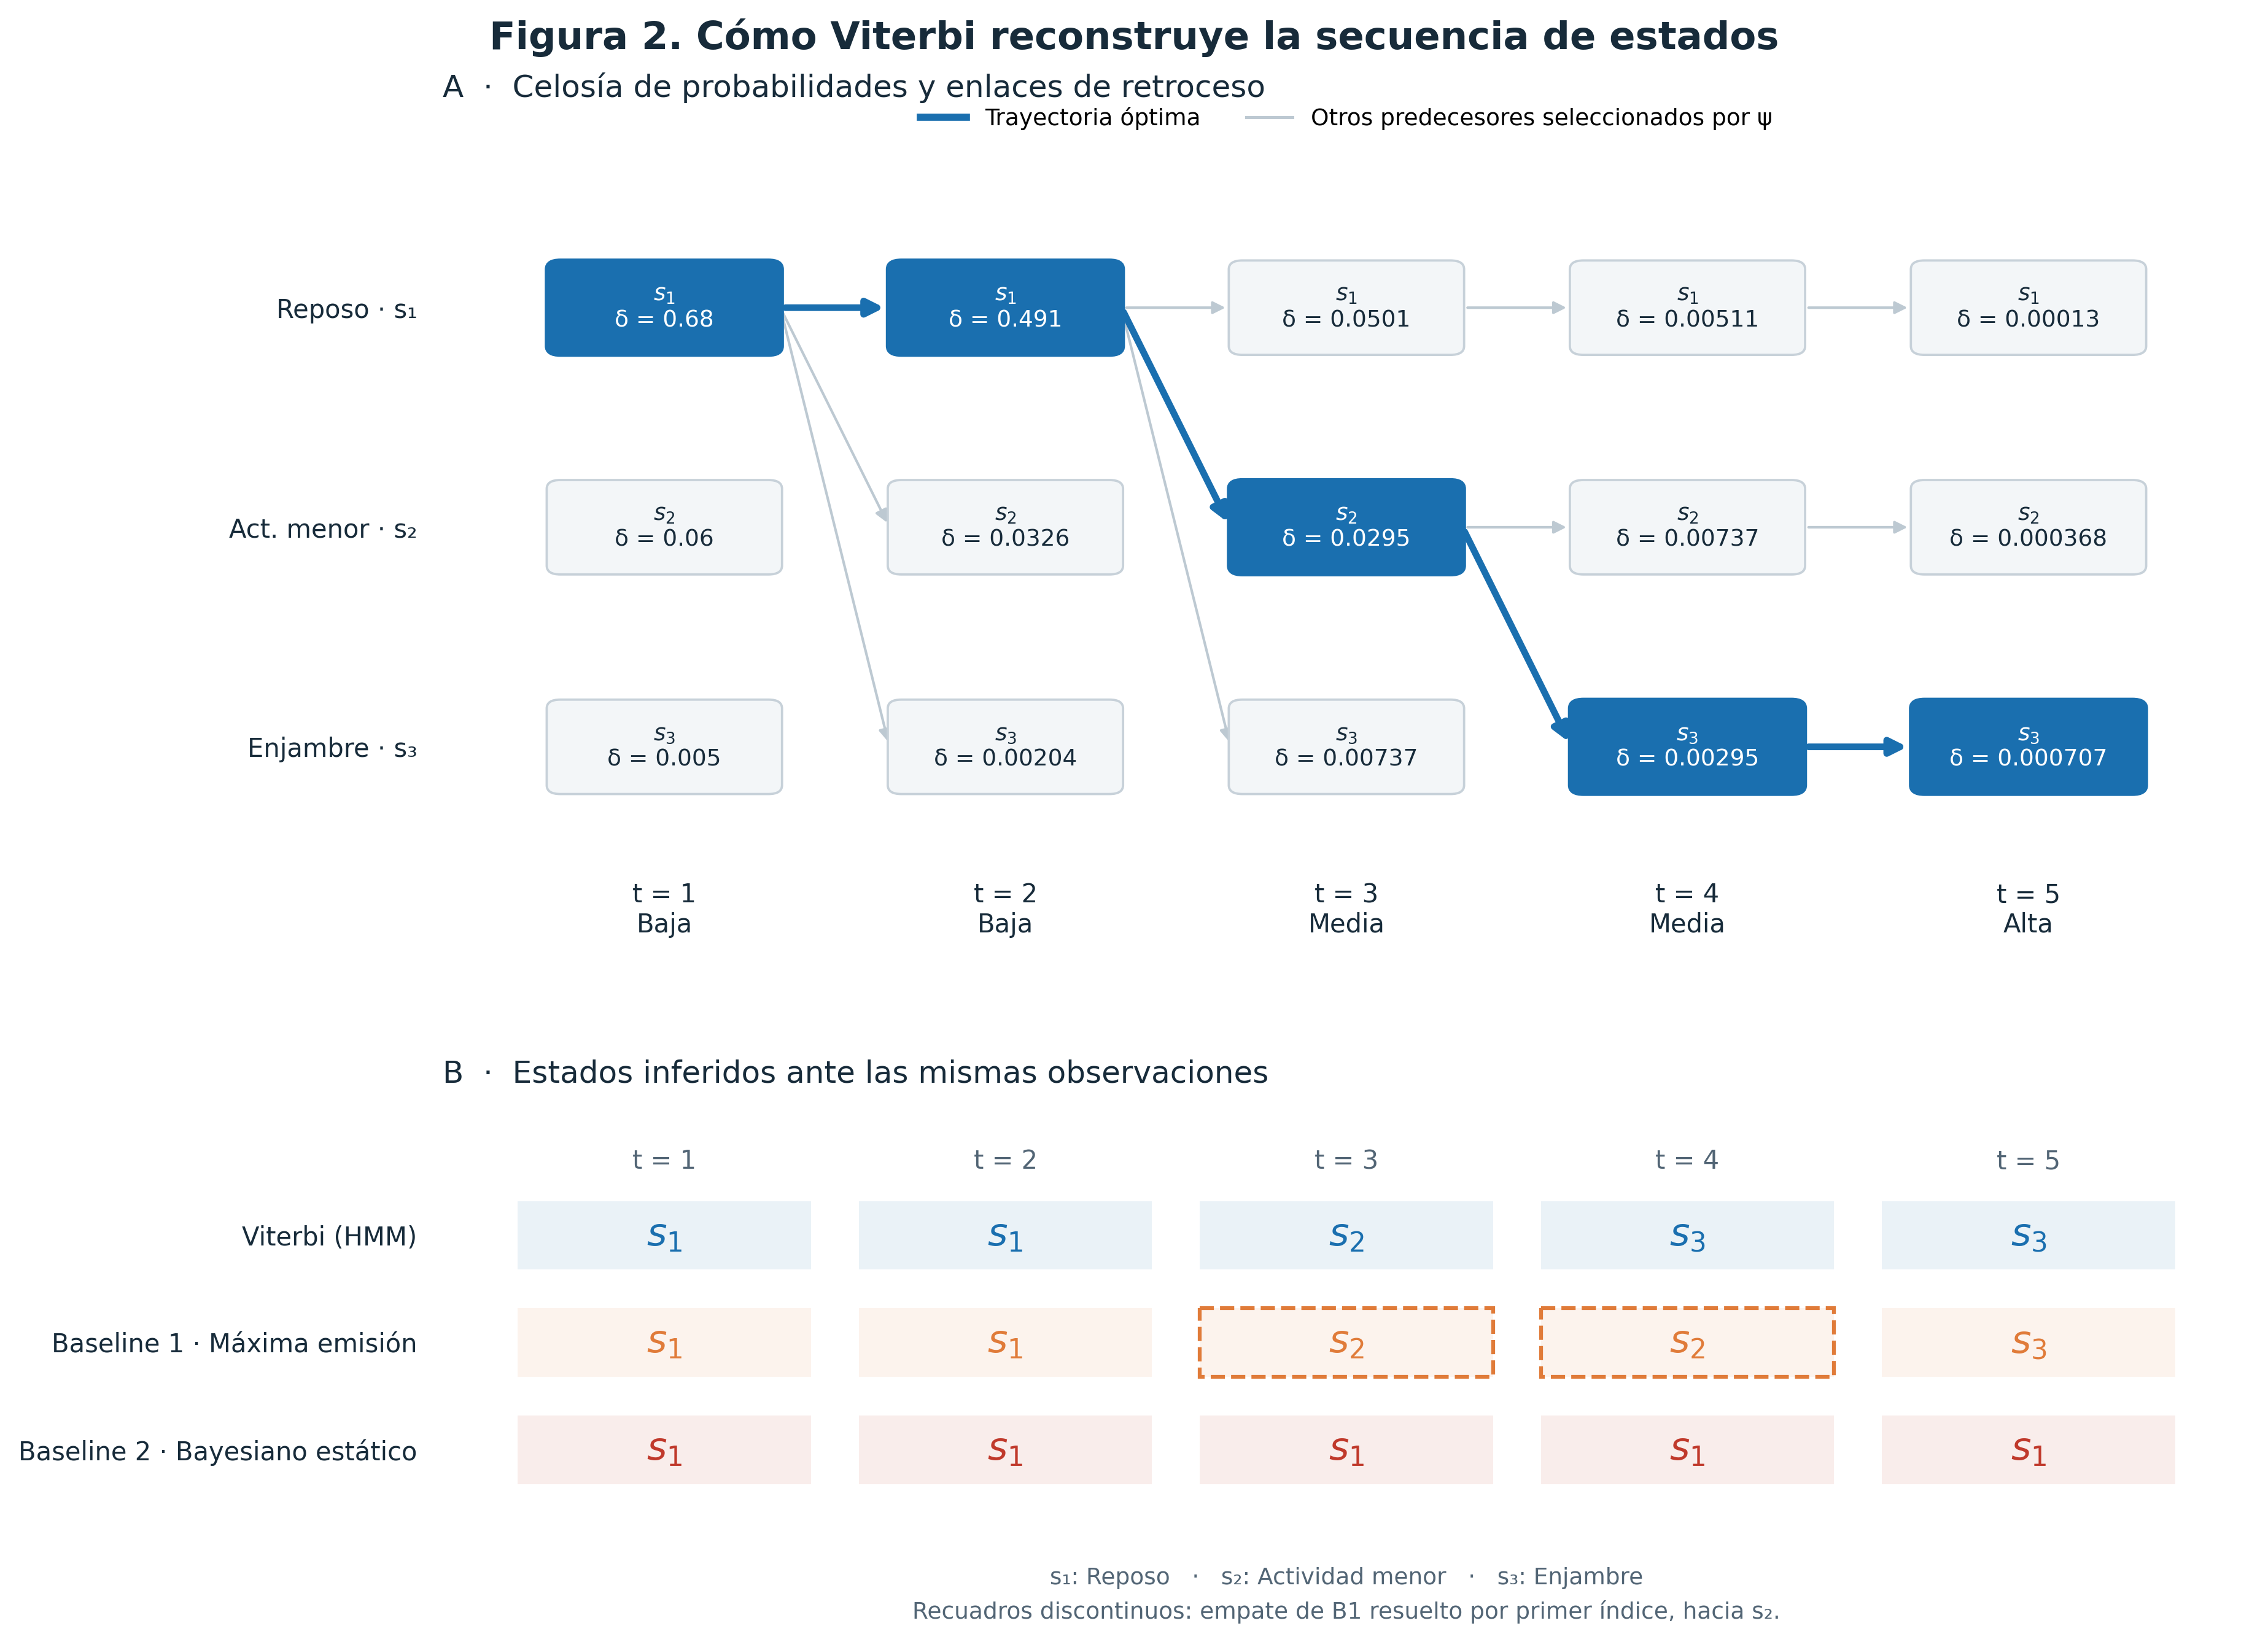
\includegraphics[width=\textwidth]{figures/fig2_celosia_viterbi.png}
\caption{Panel A: celosía con valores $\delta_t$ y enlaces seleccionados por $\psi$; el camino óptimo aparece en azul. Panel B: estados inferidos por cada método; los recuadros discontinuos marcan los empates de B1 resueltos por primer índice hacia $s_2$.}
\label{fig:celosia}
\end{figure}

La Tabla~\ref{tab:comparacion_secuencia} compara las trayectorias devueltas por los métodos. No se calcula exactitud para este caso ilustrativo porque no se conocen estados verdaderos.

\begin{table}[htbp]
\centering
\small
\caption{Trayectorias y log-probabilidad conjunta en la secuencia base.}
\label{tab:comparacion_secuencia}
\begin{tabular}{lcr}
\toprule
Método & Trayectoria inferida & $\ln P$ \\
\midrule
Algoritmo de Viterbi & $(s_1, s_1, s_2, s_3, s_3)$ & -7.2538 \\
Baseline 1 (Máxima Emisión) & $(s_1, s_1, s_2, s_2, s_3)$ & -7.4361 \\
Baseline 2 (Bayesiano Estático) & $(s_1, s_1, s_1, s_1, s_1)$ & -8.9453 \\
\bottomrule
\end{tabular}
\end{table}

\begin{figure}[htbp]
\centering
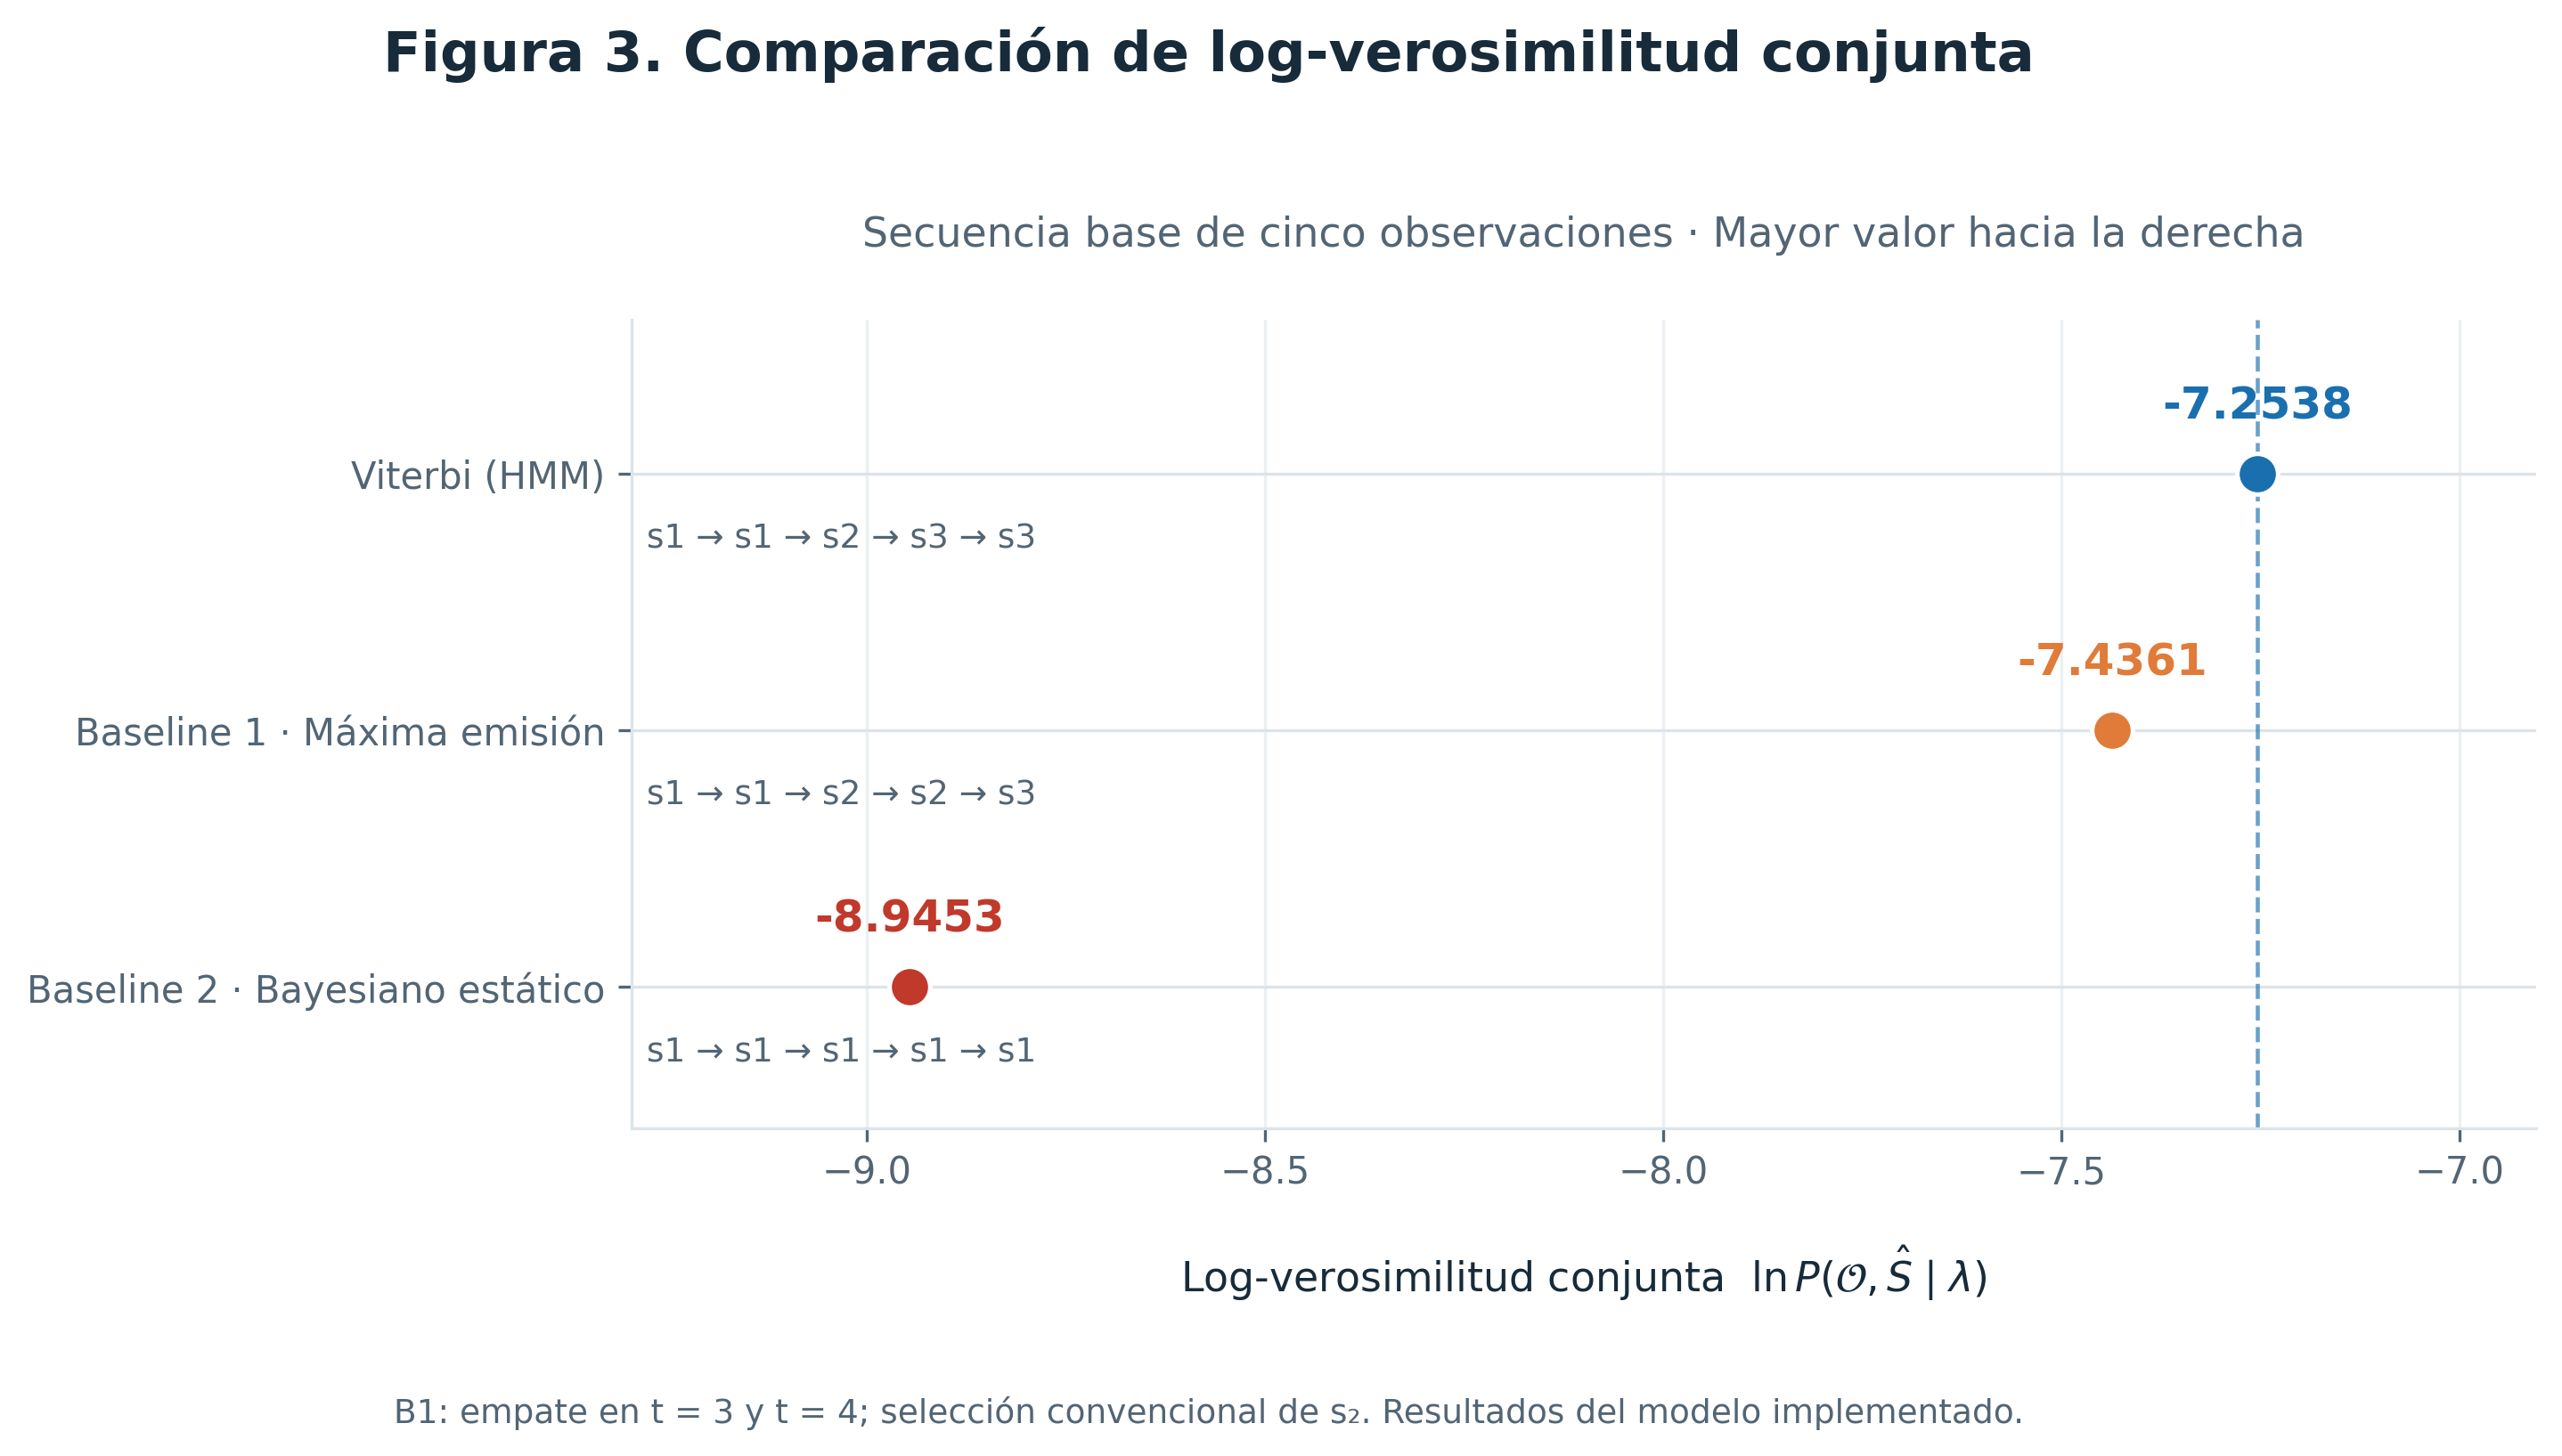
\includegraphics[width=\textwidth]{figures/fig3_comparacion_logp.png}
\caption{Log-verosimilitud conjunta: Viterbi ($-7.2538$), B1 ($-7.4361$) y B2 ($-8.9453$). Los valores mayores se sitúan a la derecha. B1 aplica el mismo desempate hacia $s_2$ utilizado en Monte Carlo.}
\label{fig:logp}
\end{figure}

\subsection{Evaluación Estadística mediante Simulación Monte Carlo ($N=100,T=50$)}

Se generaron 100 secuencias de 50 eventos con \texttt{RandomState(42)}, sorteando estado y emisión de forma intercalada. Los tres métodos evaluaron las mismas secuencias. La unidad independiente es la secuencia, no cada uno de los 5000 eventos. La Tabla~\ref{tab:monte_carlo} usa desviación muestral e intervalos normales aproximados:
\begin{equation}
IC_{95\%}=\bar{X}\pm1.96\frac{s}{\sqrt{100}}.
\end{equation}

\begin{table}[htbp]
\centering
\small
\caption{Exactitud por secuencia: resumen de las 100 réplicas.}
\label{tab:monte_carlo}
\begin{tabular}{lrrrrl}
\toprule
Método & Media & $s$ & Mínimo & Máximo & $IC_{95\%}$ \\
\midrule
Algoritmo de Viterbi & 0.7262 & 0.1094 & 0.4200 & 0.9400 & [0.7048, 0.7476] \\
Baseline 1 (Máxima Emisión) & 0.6972 & 0.0839 & 0.4800 & 0.8800 & [0.6807, 0.7137] \\
Baseline 2 (Bayesiano Estático) & 0.6154 & 0.1518 & 0.3000 & 0.9200 & [0.5856, 0.6452] \\
\bottomrule
\end{tabular}
\end{table}

Viterbi obtuvo una precisión media de $72.62\%$, frente a $69.72\%$ de B1 y $61.54\%$ de B2: diferencias de 2.90 y 11.08 puntos porcentuales. Los intervalos individuales de Viterbi y B2 no se solapan; no se calculó una prueba de hipótesis pareada ni un valor p. La desviación de Viterbi ($s=0.1094$) supera la de B1 ($s=0.0839$) y es menor que la de B2 ($s=0.1518$).

\begin{figure}[htbp]
\centering
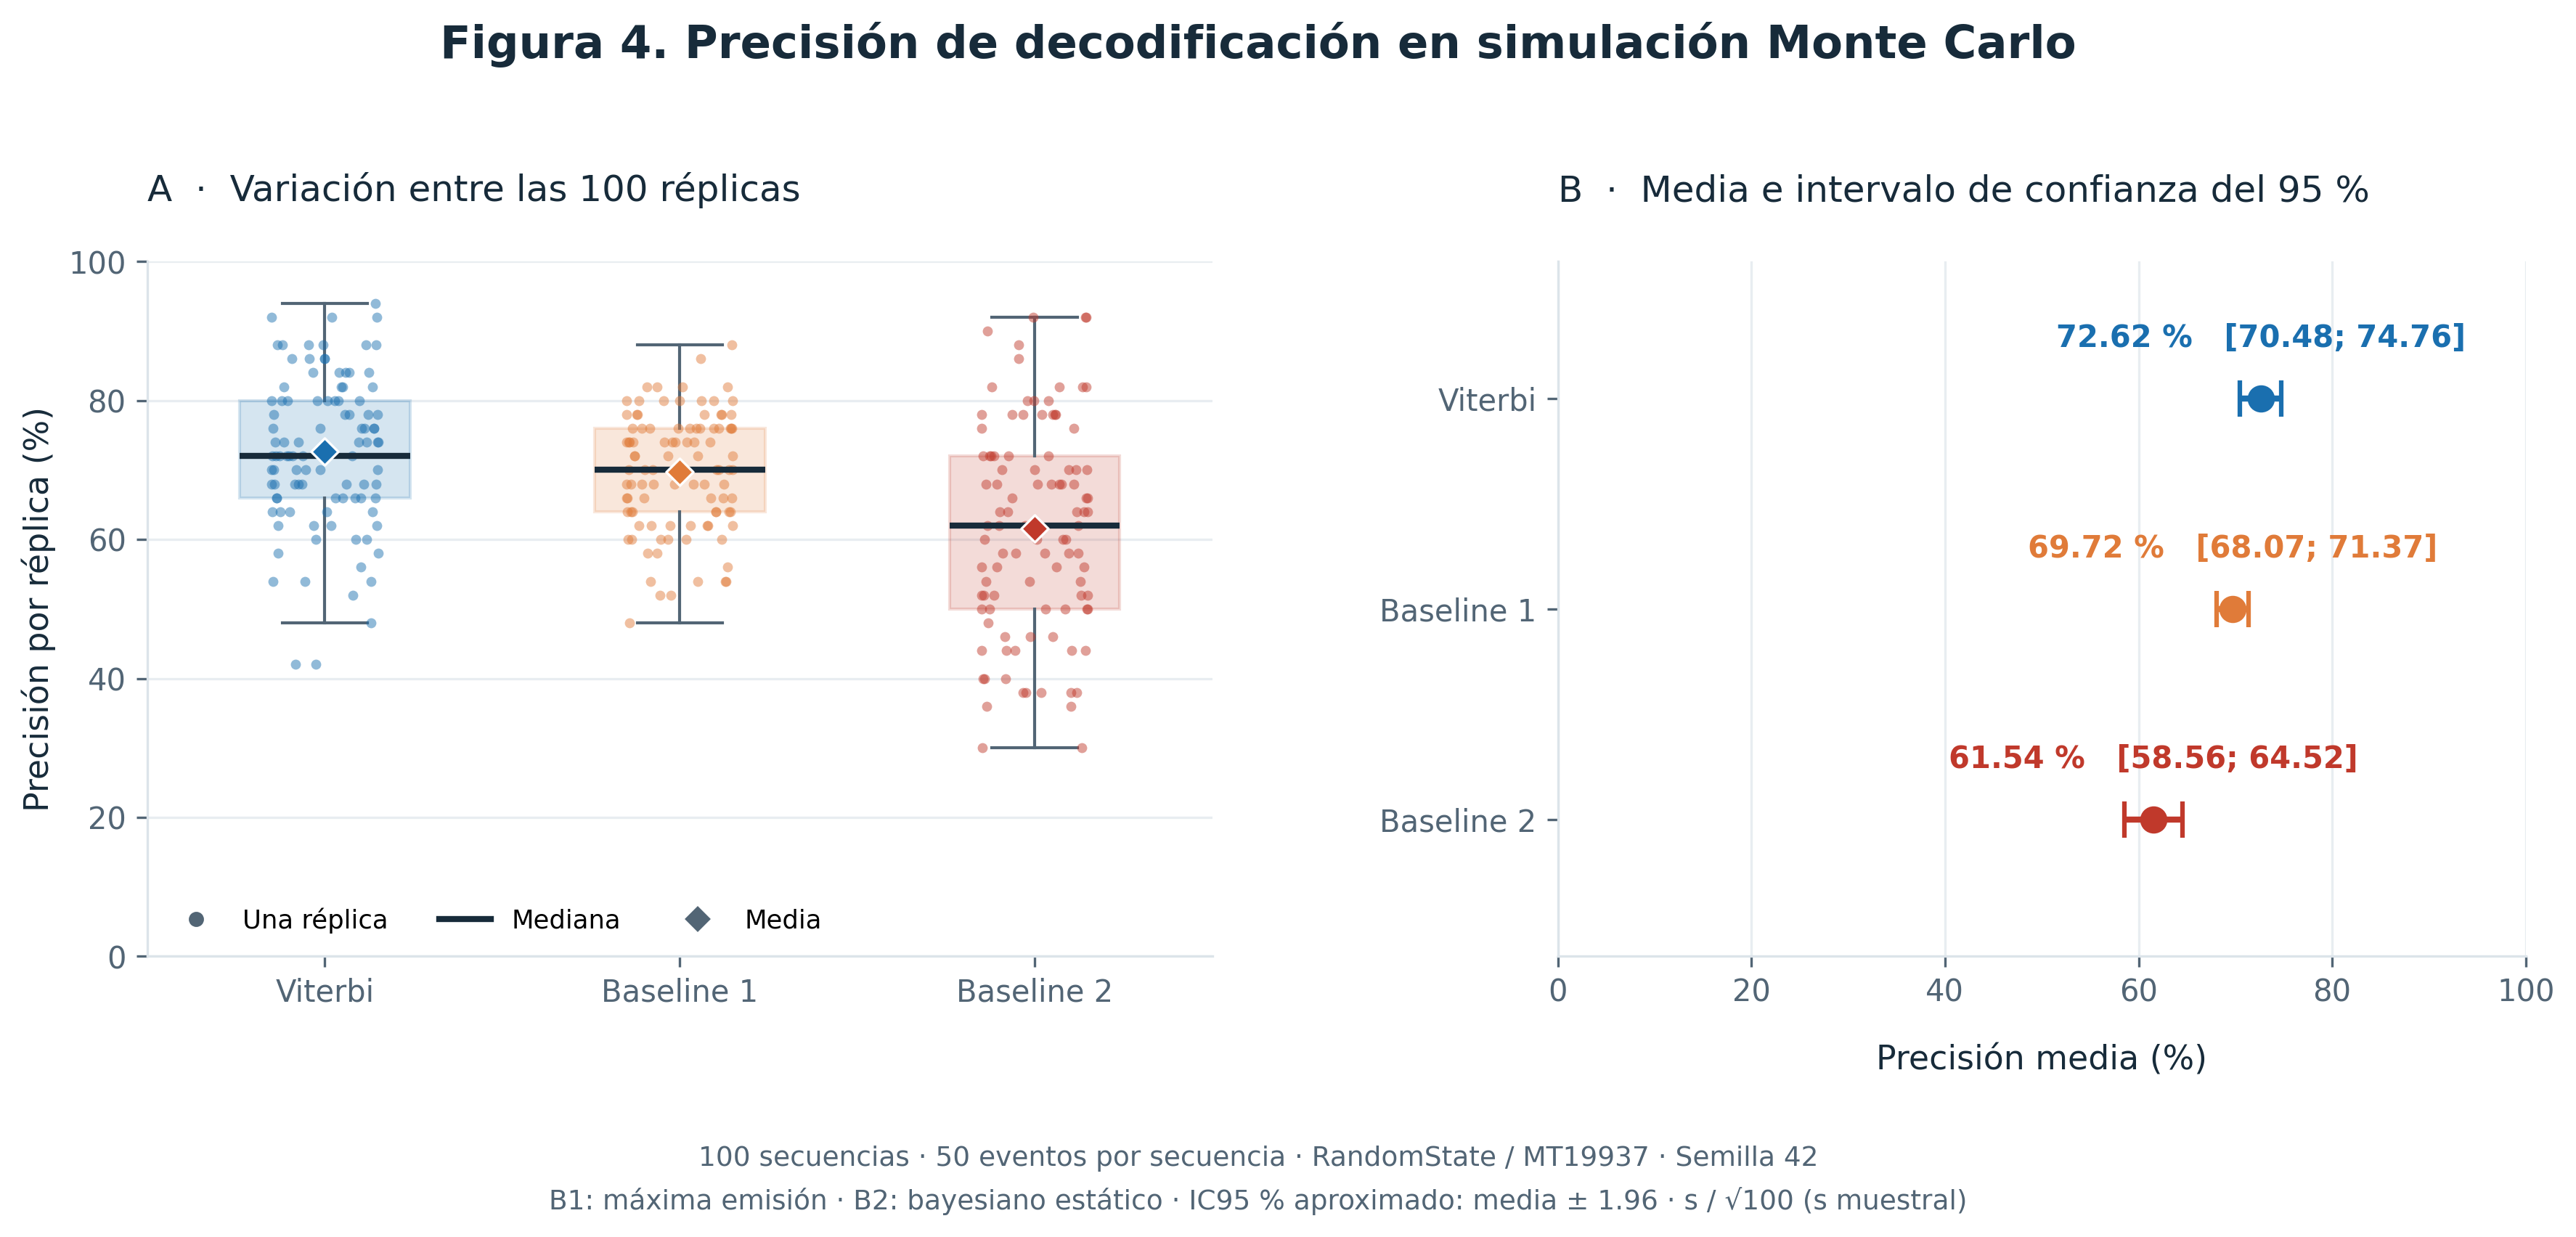
\includegraphics[width=\textwidth]{figures/fig4_monte_carlo_boxplot.png}
\caption{Panel A: distribución de exactitudes por réplica, mediana y media. Panel B: medias e intervalos aproximados del 95\%, calculados con desviación muestral. Viterbi: $72.62\%$ e IC $[70.48\%,74.76\%]$; B1: $69.72\%$ e IC $[68.07\%,71.37\%]$; B2: $61.54\%$ e IC $[58.56\%,64.52\%]$.}
\label{fig:montecarlo}
\end{figure}

Las salidas completas se conservan en \texttt{resultados/experimento.json}, \texttt{resultados/monte\_carlo.csv} y \texttt{resultados/secuencias.csv}. Los índices de estados y observaciones en estos archivos comienzan en cero.

\section{Discusión}

\subsection{Distinción entre Hallazgo e Interpretación Algorítmica}

Es fundamental distinguir rigurosamente entre los hallazgos computacionales reproducibles y su interpretación conceptual:
\begin{itemize}
    \item \textbf{Hecho verificado:} Ante una observación intermedia ($v_2$), la matriz de emisión presenta idéntica verosimilitud para actividad menor y enjambre ($B_{2,2} = B_{3,2} = 0.50$). El clasificador puntual carece de criterio probabilístico para desempatar.
    \item \textbf{Interpretación algorítmica:} El algoritmo de Viterbi resuelve esta indeterminación no por azar, sino porque incorpora la historia previa mediante el término $\delta_{t-1}(i) \cdot A_{i,j}$. Dado que la transición de Reposo a Actividad Menor ($A_{1,2} = 0.12$) es cuatro veces más probable que la transición directa a Enjambre ($A_{1,3} = 0.03$), la trayectoria inferida reconstruye la aceleración física gradual.
\end{itemize}

\subsection{Contraste con la Literatura Sismológica Contemporánea}

Los resultados corroboran los postulados de Georgakopoulou et al.~\cite{georgakopoulou2024seismic} y Allen y Wang~\cite{allen2023hidden} en cuanto a que los modelos markovianos superan a los diagnósticos estáticos en la caracterización de regímenes tectónicos no observables. Sin embargo, este trabajo añade un matiz metodológico crítico: mientras que los estudios en catálogos empíricos tienden a evaluar exactitud sobre supuestos a menudo no verificables, en este entorno controlado se comparan métodos completos: el Baseline 2 obtiene una precisión media de $61.54\%$, sin que esta comparación permita atribuir la diferencia exclusivamente al prior.

\subsection{Cuestionamiento de Explicaciones Alternativas y Límites del Estudio}

Viterbi utiliza las transiciones y la secuencia completa, mientras que los baselines clasifican cada observación por separado. La precisión media mayor no demuestra una menor dispersión: Viterbi tiene $s=0.1094$, B1 $s=0.0839$ y B2 $s=0.1518$. No se ejecutaron escenarios de sensibilidad ni una prueba pareada que permitan generalizar la ventaja observada.

\noindent \textbf{Límites del estudio:} En la geodinámica real, los ciclos sísmicos presentan memoria de largo plazo caracterizada por la acumulación y relajación de esfuerzos viscoelásticos que violan la propiedad markoviana de primer orden. Por ende, los resultados aquí obtenidos demuestran la consistencia de la técnica de programación dinámica en sistemas discretos, pero no deben extrapolarse como una herramienta de pronóstico sismológico operacional sin incorporar variables geofísicas continuas y leyes constitutivas de fricción.

\section{Conclusiones}

El presente estudio evaluó de manera cuantitativa y rigurosa el aporte metodológico del algoritmo de Viterbi en un Modelo Oculto de Markov frente a clasificadores puntuales estáticos, concluyendo:

\begin{enumerate}
    \item En la secuencia representativa base ($T=5$), el algoritmo de Viterbi resolvió de forma probabilística determinista el empate exacto ($P=0.50$) generado por la observación de magnitudes intermedias, infiriendo la trayectoria de transición gradual $(\text{Reposo}, \text{Reposo}, \text{Actividad Menor}, \text{Enjambre}, \text{Enjambre})$ con una log-verosimilitud conjunta máxima de $-7.2538$.
    \item Los clasificadores estáticos exhibieron fallas estructurales severas: el clasificador reactivo necesitó un desempate convencional hacia $s_2$ ante observaciones medias, y el clasificador bayesiano colapsó sistemáticamente en reposo constante por la influencia desmedida del prior ($\pi_1 = 0.80$, log-verosimilitud de $-8.9453$).
    \item En la simulación Monte Carlo ($N=100, T=50$), Viterbi alcanzó una precisión media de decodificación del $72.62\%$ con un intervalo de confianza al 95\,\% de $[70.48\%, 74.76\%]$, obteniendo una precisión media mayor que la del clasificador bayesiano estático ($61.54\%$, $IC_{95\%} = [58.56\%, 64.52\%]$) y aventajando en 2.90 puntos porcentuales al clasificador por máxima emisión. Estas diferencias son descriptivas; no se calculó una prueba pareada de significancia.
    \item La modelación de transiciones de primer orden permite incorporar dependencia temporal en la decodificación retrospectiva de estos escenarios sintéticos. Este resultado no establece validez física ni capacidad predictiva sobre sismos reales.
\end{enumerate}

\section*{Declaraciones}

\subsection*{Declaración de Uso de Inteligencia Artificial Generativa y Tecnologías Asistidas}
Durante la preparación de este trabajo, el autor utilizó modelos de lenguaje basados en inteligencia artificial con propósitos exclusivos de asistencia técnica en redacción formal en sintaxis LaTeX y optimización tipográfica del manuscrito. La formulación conceptual, la arquitectura del diseño de simulación, la ejecución de las suites de código en Python, el análisis de los intervalos de confianza y las conclusiones derivadas fueron concebidas, revisadas, ejecutadas y auditadas íntegramente por el autor bajo la supervisión del docente asesor.

\subsection*{Disponibilidad de Datos y Materiales de Reproducibilidad}
El código fuente en Python (\texttt{run\_viterbi\_caso.py}), la suite de pruebas unitarias (\texttt{tests/test\_stochastic.py}), el archivo de dependencias (\texttt{requirements.txt}) y el archivo de citas (\texttt{referencias.bib}) son de acceso abierto e irrestricto en el repositorio local del proyecto.

\subsection*{Conflicto de Interés}
Los autores declaran que no existen conflictos de interés de carácter financiero, académico o personal que hayan influido en el diseño del estudio o en la interpretación de los resultados computacionales presentados.

% --- BIBLIOGRAFÍA ---
\bibliographystyle{IEEEtran}
\bibliography{referencias}

\appendix
\section{Estructura del Repositorio y Reproducibilidad}

Para garantizar la reproducibilidad computacional total exigida por los estándares institucionales, el repositorio se estructura formalmente como sigue:

\begin{lstlisting}[style=pythonstyle, numbers=none]
Actividad_2/
|-- README.md
|-- anteproyecto_hmm_sismico.md
|-- main.tex
|-- referencias.bib
|-- run_viterbi_caso.py
|-- generar_figuras.py
|-- requirements.txt
|-- overleaf_articulo_hmm.zip
|-- BITACORA_DECISIONES_EQUIPO.md
|-- src/
|   |-- hmm_model.py
|   `-- experimento.py
|-- scripts/
|   `-- sincronizar_articulo.py
|-- resultados/
|   |-- experimento.json
|   |-- monte_carlo.csv
|   `-- secuencias.csv
|-- figures/
|   |-- fig1_matrices_hmm.png
|   |-- fig2_celosia_viterbi.png
|   |-- fig3_comparacion_logp.png
|   `-- fig4_monte_carlo_boxplot.png
|-- sustentacion/
|   |-- presentacion.html
|   |-- guion.md
|   `-- README.md
|-- tests/
|   |-- test_stochastic.py
|   |-- test_experimento.py
|   `-- test_documentacion.py
|-- docs/
|   `-- superpowers/plans/
`-- materiales/
    |-- caso-sismico.md
    |-- articulo.pdf
    |-- articulo_hmm_sismico_openalex.pdf
    |-- articulo_openalex_sismico.pdf
    `-- stats-07-00047.pdf
\end{lstlisting}

\section{Guion Estructurado para la Sustentación Oral (Video Pitch 4--5 Minutos)}

El guion completo y la presentación HTML se conservan en \texttt{sustentacion/guion.md} y \texttt{sustentacion/presentacion.html}. Las ocho diapositivas siguen los cuatro bloques de esta pauta y permiten una exposición individual de aproximadamente 4 minutos y 30 segundos.

Para la presentación del trabajo, se diseñó la siguiente pauta temática individual con marcas de tiempo rigurosas y parlamentos sugeridos para el autor \textbf{Francisco Javier Florez Ramirez}:

\begin{table}[htbp]
\centering
\small
\caption{Estructura de sustentación oral individual del autor.}
\begin{tabular}{p{2.2cm}p{4.5cm}p{2.8cm}p{3.5cm}}
\toprule
\textbf{Bloque} & \textbf{Eje Temático} & \textbf{Intervalo Tiempo} & \textbf{Apoyo Visual} \\
\midrule
Bloque 1 & Contexto, Problema y Pregunta Central & 0:00 – 1:00 (60 s) & Diapositivas 1 y 2 \\
Bloque 2 & Formalismo HMM y Baselines de Control & 1:00 – 2:05 (65 s) & Diapositivas 3 y 4 \\
Bloque 3 & Algoritmo Viterbi y Resultados Clave & 2:05 – 3:20 (75 s) & Diapositivas 5 y 6 \\
Bloque 4 & Discusión, Límites y Conclusiones & 3:20 – 4:30 (70 s) & Diapositivas 7 y 8 \\
\bottomrule
\end{tabular}
\end{table}

\noindent \textbf{Parlamento sugerido (Apertura):} \\
\textit{«Cordial saludo profesor y evaluadores. Mi nombre es Francisco Javier Florez Ramirez, estudiante de Ingeniería de Software y Datos de la IU Digital de Antioquia, y bajo la asesoría del docente Dr. Julián Andrés Loaiza López, presento la evaluación experimental del Algoritmo de Viterbi frente a clasificadores estáticos para la inferencia de regímenes de actividad sísmica latente...»}

\end{document}
